\documentclass[hyperref,UTF8]{ctexart}    
	\usepackage{amsmath}
	\usepackage{amssymb}	
	\usepackage[a4paper,bindingoffset=0.2in,%
            left=1in,right=1in,top=1in,bottom=1in,%
            footskip=.25in]{geometry}
\usepackage{graphicx}
\usepackage{enumerate}
\usepackage{url}
\usepackage{hyperref}
\usepackage{pbox}
\usepackage{CJKutf8}


\begin{document}
\title{ASS2实验报告}
\author{盛嘉成, 14307130038 \\ 计算机科学与技术学院}
\maketitle

\section*{PCA}
使用PCA将高维的数据映射到低维的子空间,实现特征提取、压缩等目的。如果以最大方差的角度考虑PCA,那么映射的目的是把原数据映射到一个主子空间(principle subspace),以使得映射后的数据方差最大。因为方差越大,某种程度上意味着保留的信息越多。
以映射到一维为例,目标是最大化下式:
\[\frac{1}{N}\sum_{n=1}^{N}(\omega^T x_n-\omega^T\bar x)^2\]
其中规定$\omega$为单位向量(否则最大化上式可能导致最大化$\omega$,而我们只关注其方向),为了满足$\omega^T\omega=1$的限制,加入拉格朗日乘数,最大化下式:
\[\omega^T S \omega + \lambda(1-\omega^T\omega)\]
其中$S=\frac{1}{N}\sum_{n}(x_n-\bar x)(x_n-\bar x)^T$是训练集的协方差矩阵。
令其导数为0,有:
\[S\omega = \lambda \omega\]
所以$\omega$为S的一个特征值,又:
\[\omega^T S \omega = \lambda\]
所以最大方差对应着S最大的特征值,取对应的特征向量就是$\omega$。
\par 要映射到D维空间时,只需要取S前D大的几个特征值对应的特征向量即可。
\subsection*{可视化}\ 
\par训练集映射到2维或3维的效果:\\
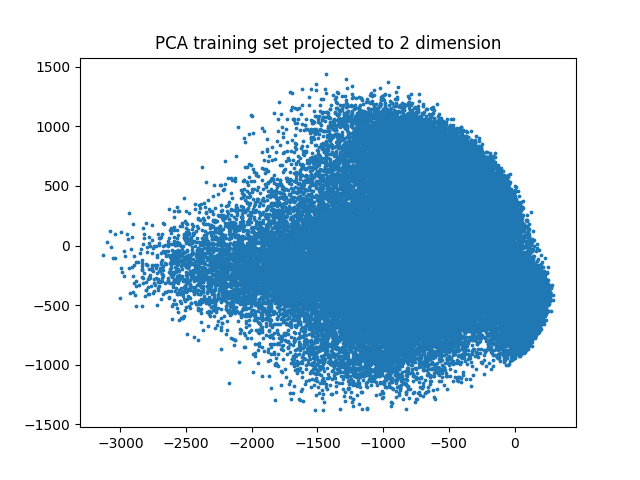
\includegraphics[height=4.2in]{exp-results/pca2.png}\\
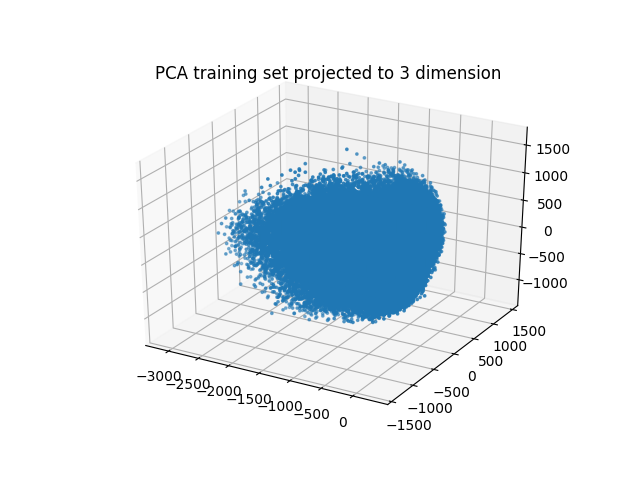
\includegraphics{exp-results/pca3.png}\\
\par 单单从这两幅图中没能得到太多直观信息。
\par 将3维主子空间(前三大的特征值对应的特征向量)重新转换成28*28的图片:\\
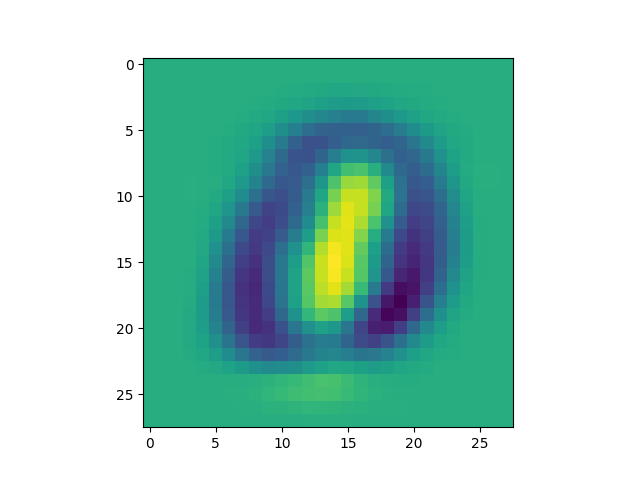
\includegraphics[height=2.9in]{exp-results/eign0.png}\\
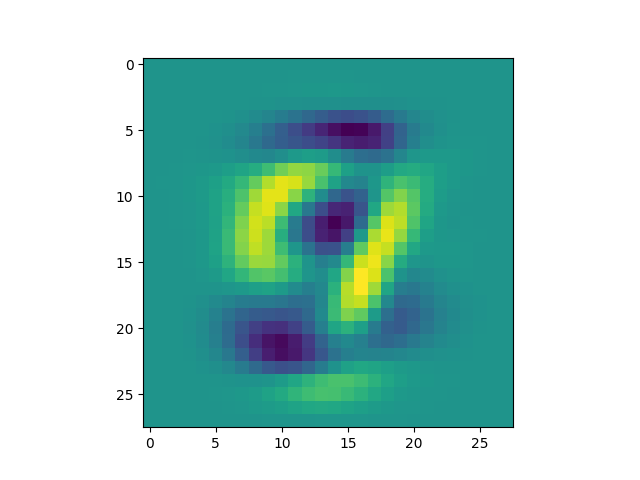
\includegraphics[height=2.9in]{exp-results/eign1.png}\\
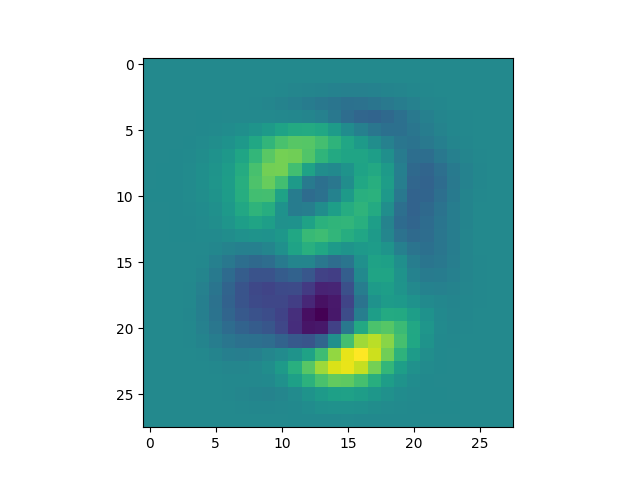
\includegraphics[height=2.9in]{exp-results/eign2.png}\\
\par 特征向量的可视化非常成功,定性的来看,特征向量中值比较大的位置(在子空间更有影响力的像素)基本上就是手写数字笔画覆盖比较集中的位置。
\subsection*{最近邻分类}\
\begin{table}[!htbp]
% \resizebox{1.4\linewidth}{!}
  \centering
  \scalebox{1}{
\begin{tabular}{ l || c | c | c }
  \hline      
  dimension & 40 & 80 & 200  \\ \hline
  accuracy \%  & 97.25 & 97.34 &96.85 \\
  \hline  
\end{tabular}
}
\caption{PCA不同维度下NN分类准确率}
\label{tb:lda_knn}
\end{table}
\par 提取较少维度的主成分就可以得到很好的分类效果(额外实验发现即使只有10维的情况下也能有$90.8\%$的准确率)。这一方面说明采用最大方差准则进行降维的PCA确实可以比较好的保留信息,另一方面,更说明了对于图片这样的高维数据和识别的任务而言,很多维度如四周空白位置的像素信息是没有实际信息量的,所以大大压缩后还能有很好的分类表现。
\subsection*{维度选取}\
\par 样本数据空间M维,那么协方差矩阵的M个特征值之和称为总能量,而提取的前d个特征值之和就是主子空间保留的能量。
\par 在本次实验的数据上,149维的主成分就可以保留$95\%$的总能量,此时的分类准确率为$97.02\%$
\par 降维到多少维的子空间合适其实没有固定的选取方法,除了限定保留的能量(或者等价的失真度$J=\sum_{i=d+1}^{M}\lambda_i$),也可以设定阈值,丢掉对应特征值较小的维度。如果作为分类的预处理,那么可以结合分类错误率选择,如果是压缩图像的任务,那么直接根据需要压缩率选择d即可。



\section*{LDA}
\par LDA本质就是Fisher线性判别模型,虽然也是把数据进行降维,但是和PCA不同,PCA是把数据压缩,希望在低维的子空间上尽可能保留原数据的信息,而LDA是为分类服务的,带监督的模型,其目的是找到一个低维空间,使得投影后的不同类数据尽可能能被区分。
\par 以二分类的情况为例,首先一个很自然的考虑是两类别数据投影后的均值距离$m_1-m_2=\omega^T(\sum_{n\in C_1}x_n/N_1-\sum_{n\in C_2}x_n/N_2)$越远越好,但实际上可能存在均值距离达到最大但两类的重叠很严重的情况,所以增加一个标准:令每个类别内部的方差较小以减小类间的重叠。于是根据Fisher准则,找各类能被更好分开的子空间,可以通过最小化以下函数解决:
\[J(\omega)=\frac{\omega^T S_B \omega}{\omega^T S_W \omega}\]
其中$S_B$是类间协方差矩阵,$S_W$为类内协方差矩阵,满足约束$\omega^T\omega=I$。
\par 多分类情况下:
\[S_W = \sum_{k=1}^{K}\sum_{n\in C_k}(x_n-m_k)(x_n-m_k)^T\]
\[S_B=\sum_{k=1}^{K}N_k(m_k-m)(m_k-m)^T\]
其中m为全体数据的均值。
\par 前d大的目标函数取值,对应$S_{W}^{-1}S_B$的前d大的特征值,此时的$\omega$即由相应的d个特征向量组成。
\par 在本次实验的具体实现中遇到两个小问题,首先是面对如此大的训练样本数量计算$S_W$会非常慢,而更棘手的是算法其实隐含了对$S_W$可逆的假设,但这个假设并不总是成立,在MNIST数据集上,10类图片全部样本最周围位置的像素取值总是为0,即很多维度上类内方差为0,$S_W$很多行列全0,是奇异阵,不能直接按照原算法求逆。对于这一问题有两个解决办法,一种是去掉这些为定值的维度,因为显然这些维度在任何分类方法中都不会有贡献,二是改用$S_{W}^{-1}S_B$的伪逆矩阵代替。(本次实验选择了第二种方法)
\subsection*{可视化}\
训练集映射到2维或3维的效果:\\
\centerline{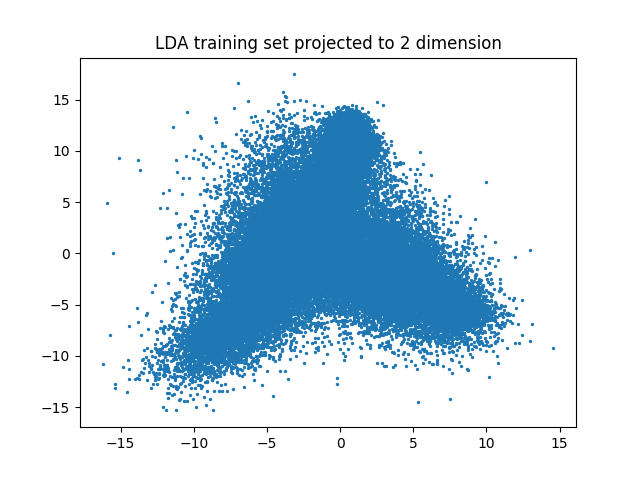
\includegraphics[height=3.6in]{exp-results/lda2.png}}
\centerline{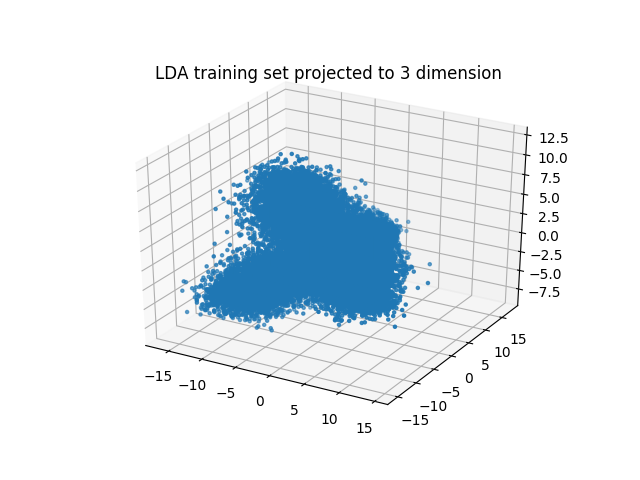
\includegraphics[height=4in]{exp-results/lda3.png}}
\par 与PCA不同,使用LDA降维后不同类的数据能分开,同类会“抱团”。虽然图中没有显示样本的标签,但我们也能大致观察到一簇簇聚集的效果(取少一点样本可以更清晰地观察到)
\centerline{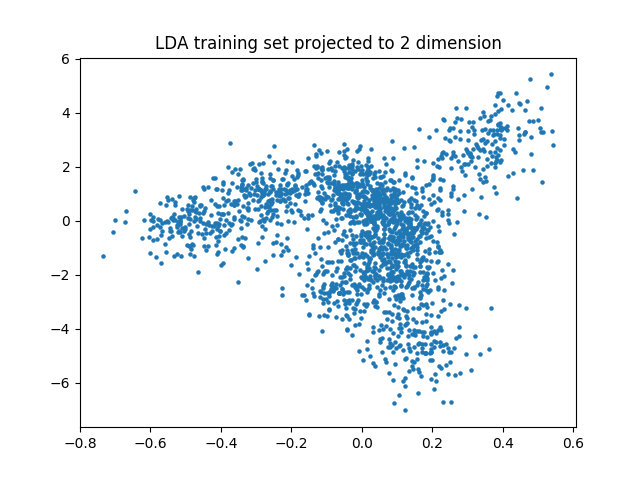
\includegraphics[height=2.4in]{exp-results/lda2test.png}}
\par 特征值的可视化:\\
\centerline{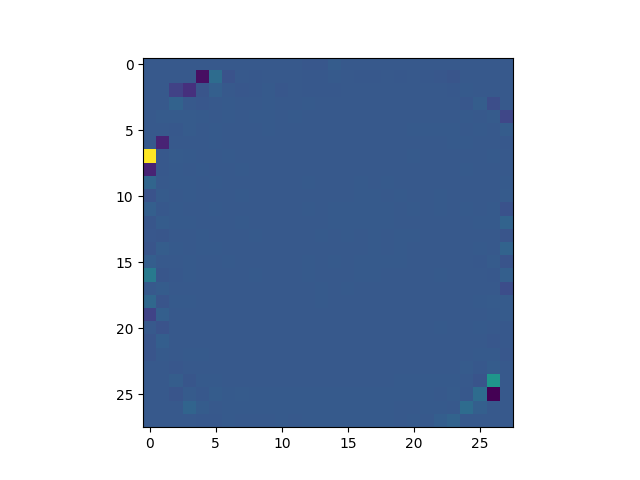
\includegraphics[height=2.1in]{exp-results/ldaeig0.png}}
\centerline{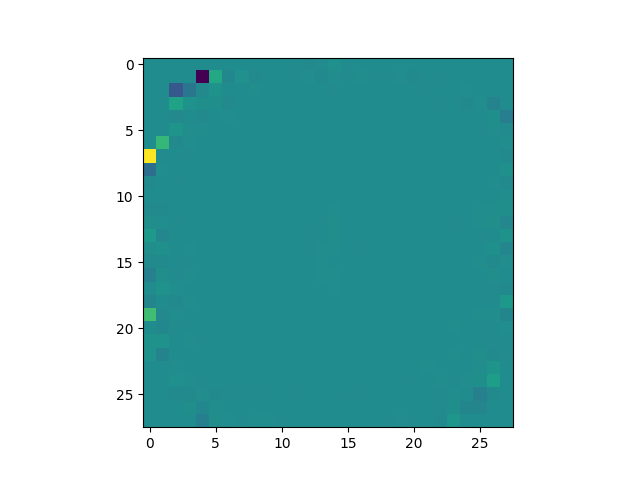
\includegraphics[height=2.1in]{exp-results/ldaeig1.png}}
\par 与PCA不同,构成LDA低维映射空间的特征值本身可视化后是看不出任何直观意义的。
\subsection*{最近邻分类}\
\begin{table}[!htbp]
  \centering
  \scalebox{1}{
\begin{tabular}{ l || c | c | c }
  \hline      
  dimension & 2 & 3 & 9  \\ \hline
  accuracy \%  & 47.41 & 66.64 &89.5 \\
  \hline  
\end{tabular}
}
\caption{LDA不同维度下NN分类准确率}
\label{tb:lda_knn}
\end{table}
\par 虽然表明上看2维,3维的成功率不算很高,但对于10分类问题,这样的准确率是可以接受的。而提高到9维(实际最高能映射到9维),就得到了九成的准确率。为了说明LDA在极大降维率的情况下,区分开各类样本的效果,可以和PCA在同样维度数下分类作对比:\\
\begin{table}[!htbp]
% \resizebox{1.4\linewidth}{!}
  \centering
  \scalebox{1}{
\begin{tabular}{ l || c | c | c }
  \hline      
  dimension & 2 & 3 & 9  \\ \hline
  accuracy \%  & 38.75 & 47.66 &89.17 \\
  \hline  
\end{tabular}
}
\caption{PCA同样维度下准确率}
\label{tb:lda_knn}
\end{table}
\par 在只有2或3维时,PCA明显不如LDA的效果,这和我们把降维后数据可视化的结果是一致的。

\subsection*{基于类均值分类}\
\par 实际上,我并不十分赞同作业中布置的LDA+最近邻的分类方法,原因有二,一是对于60000个训练样本,即使在低维空间,找最近邻也需要相当大的时间代价。二是LDA既然把各类样本在低维空间分开了,那采用最近邻分类其实在某种程度上浪费了每个类的样本分别抱团后的良好整体特性,而让分类只关注每个测试样本周围的局部空间,容易受干扰。
\par 所以我额外尝试了一种分类方法,即找低维空间中里自己最近的各类的类内均值点(10个),这样一来每个测试样本只要计算10次距离而不是60000次,二来也充分利用的Fisher准则。实际的效果不仅时间上大大加快,在极低维度时分类准确率也胜过最近邻:
\begin{table}[!htbp]
% \resizebox{1.4\linewidth}{!}
  \centering
  \scalebox{1}{
\begin{tabular}{ l || c | c | c }
  \hline      
  dimension & 2 & 3 & 9  \\ \hline
  accuracy \%  & 54.67 & 69.95 &86.93 \\
  \hline  
\end{tabular}
}
\caption{LDA基于最近均值点分类}
\label{tb:lda_knn}
\end{table}

\subsection*{能映射的最高维}\
\par 对于K个分类,LDA能找到的子空间至多不会超过K-1维,原因是$S_B=\sum_{k=1}^{K}N_k(m_k-m)(m_k-m)^T$由K个矩阵的和组成,每一个矩阵都是两个向量的外积,因此每个秩等于1。
\par 又有如下限制条件,
\[\sum_{k=1}^{K}N_km_k=\sum_{n=1}^{N}x_n\]
\par 所以这些矩阵中只有K-1个是相互独立的。因此$S_B$的秩最大等于K-1,因此最多$S_{W}^{-1}S_B$有K-1个非零特征值。




\section*{SVM}
\par 以二分类,样本线性可分的情况为例,样本标签$t_n \in \{-1,1\}$,线性SVM大致思想是找到一个分类的决策面$y(x)=\omega^T\phi(x)+b$,不仅满足$t_n y(x_n)>0$(正确分类训练集样本),而且希望能最大化样本和这个决策面的最近距离(margin),即:
\[{\arg\max}_{\omega,b}(\frac{1}{\|{\omega}\|}{\min}_n[t_n(\omega^T\phi(x_n)+b)])\]
令距离决策面最近的点满足:
\[t_i(\omega^T\phi(x_i)+b) = 1\]
这样就限制对所有样本:
\[t_n(\omega^T\phi(x_n)+b) \ge 1\]\[(n = 1,2,,,N)\]
\par 于是原问题就等价于在限制条件下最小化${\|\omega\|}^2$。
\par 为了计算,将限制条件通过引入拉格朗日乘数来满足,即:
\[L(\omega,b,a)=\frac{1}{2}{\|\omega\|}^2-\sum_{n=1}{N}a_n(t_n(\omega^T\phi(x_n)+b)-1)  \]
\par 关于$\omega,b$最小化,关于a最大化这个拉格朗日函数,就求得了我们需要的决策面。
\par 或者,利用上式导数为零得到条件消去$\omega,b$,我们可以得到用核函数表示的,原最大化边缘问题的对偶表示,即关于a最大化:
\[L'(a)=\sum_{n=1}^{N}a_n-\frac{1}{2}\sum_{n=1}^{N}\sum_{m=1}^{N}a_n a_m t_n t_m k(x_n,x_m)\]
\par 条件为:
\[a_n\ge0,\sum_{n=1}^{N}a_n t_n =0\]
\par 线性SVM中,$k(x,x')=\phi(x)^T\phi(x')$,但其他情况下也可以使用如高斯核等其他核函数。

\subsection*{C-SVM}\
\par 而为了应对数据不是线性可分的情况,或者为了避免如下情况:\\
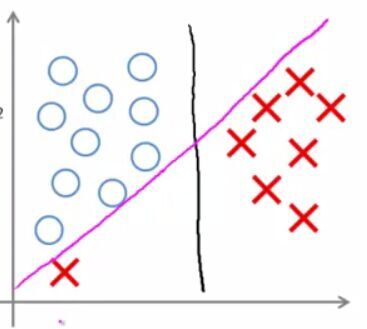
\includegraphics[height=2in]{exp-results/C-svm.jpg}
\par (线性SVM最大化margin的做法会得出红线表示的决策边界)
\par 允许训练集上的样本出现在决策边界错误的一侧,但是引入一个惩罚项。具体的我们最小化:
\[C\sum_{n=1}^{N}\xi_n + \frac{1}{2}{\|\omega\|}^2\]
\par 其中对正确分类且在决策面的边缘里内的样本,定义$\xi_n=0$,而其他点$\xi_n=|t_n-y(x_n)|$,于是$\xi_n>1$的就是被分错的点。优化决策面的限制条件变成$t_n y(x_n)\ge 1-\xi_n$
\par 当参数$C>0$越大,最小化上式意味着越不允许误分类,C趋于无穷大时,最小化上式等价于线性可分假设下的SVM

\subsection*{PCA + linear SVM}

\begin{table}[!htbp]
% \resizebox{1.4\linewidth}{!}
  \centering
  \scalebox{1}{
\begin{tabular}{ l || c | c | c | c}
  \hline      
	accuracy \% & d=40 & d=80 & d=200 & raw \\ \hline
	C=0.01  & 93.22 & 93.91 & 94.31 & 94.38\\
	C=0.1   & 93.37 & 94.31 & 94.53 & 94.69\\
	C=1     & 93.26 & 94.34 & 94.11 & 93.98\\
	C=10    & 93.24 & 94.11 & 93.61 & 93.08\\
  \hline  
\end{tabular}
}
\caption{PCA降至不同维度,SVM不同C取值的分类准确率}
\label{tb:lda_knn}
\end{table}
\par 从实验结果来看,首先C相同,维度越高,分类效果越好。这和正常直觉一致,PCA映射到的主子空间维度越低,越可能导致不同类的样本混杂在一起。
\par 从C的变化来看,大致上,分类准确率随着C的增大,先增大后减小。这是因为C过大时,SVM只强调最大化决策边缘,不容忍误分类,容易受到游离在同类之外的极小一部分样本的影响。而反过来C过小时,对误分类的惩罚项过小,过度容忍,使得最后选择的决策面不理想。

\subsection*{kernel SVM}
\par 当样本线性不可分的时候:\\
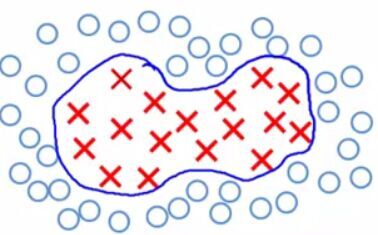
\includegraphics[height=1in]{exp-results/kernel.jpg}
\par 我们需要一个比线性基更好的,能描绘如图中所示的决策面的模型。此时可以如前文所说的替换核函数。
\par 本次实验使用了径向基核:
\[k(x,x')=exp(\gamma{\|x-x'\|}^2)\]

\par 实验效果如下:

\begin{table}[!htbp]
% \resizebox{1.4\linewidth}{!}
  \centering
  \scalebox{1}{
\begin{tabular}{ l || c | c | c | c}
  \hline      
	accuracy \% & $\gamma=0.01$ & $\gamma=0.025$ & $\gamma=0.05$ & $\gamma=0.1$ \\ \hline
	C=1     & 97.44 & 98.30 & 98.51 & 98.62\\
	C=10    & 98.44 & 98.51 & 98.55 & 98.29\\
	C=100   & 98.45 & 98.53 & 98.54 & 98.29\\
	C=1000  & 98.41 & 98.53 & 98.54 & 98.29\\
  \hline  
\end{tabular}
}
\caption{kernel SVM分类准确率}
\label{tb:lda_knn}
\end{table}
\par 上表实验中,PCA的维度固定为40维,因为维度越高,分类效果更好几乎是必然的,所以没有再在维度上进行变化并实验,而且从结果来看40维也已经足够好了。
\par 从表内的实验来看,C的选择其实随着$\gamma$不同略有不同,大致在100左右有比较好的表现。而关于$\gamma$其实有很多资料包括libsvm本身都推荐取(1/特征数),本例中即0.025,实验表明这种选择基本上合理,当然具体数据集上不一定是最好的。
\par 整体上,和线性SVM比,可以发现kernel SVM的效果明显更好,说明至少对于本次实验的训练集降低到40维后,存在一定线性不可分的情况,相对更适合用径向基核描述决策面。

\section*{survey}
用时30小时左右。

\par
\
\par PS: 非实验的图片来自machine learning(Andrew Ng)的视屏截图
\bibliographystyle{plain}
\bibliography{report}


\end{document}